\documentclass{sbmlpkgspec}

%% ============================================================================
%% Description:  Documentation for the SBML Test Runner
%% First author: Michael Hucka <mhucka@caltech.edu>
%% Organization: California Institute of Technology
%% Date created: January 2013
%%
%% Copyright (C) 2011-2013 California Institute of Technology, Pasadena, CA.
%%
%% The SBML Test Suite is free software; you can redistribute it and/or modify
%% it under the terms of the GNU Lesser General Public License as published by
%% the Free Software Foundation.  A copy of the license agreement is provided
%% in the file named "LICENSE.txt" included with this software distribution.
%% ============================================================================

% Settings just for this file

% Custom latex listing style, for use with the listings package.  The default
% highlights far too many things, IMHO.  This keeps it simple and only adjusts
% the appearance of comments within listings.

\lstdefinelanguage{mylatex}{%
  morekeywords={},%
  sensitive,%
  alsoother={0123456789$_},%$
  morecomment=[l]\%%
}[keywords,tex,comments]

\lstdefinestyle{latex}{language=mylatex}

% -----------------------------------------------------------------------------
% Start of document
% -----------------------------------------------------------------------------

\begin{document}

\packageTitle{The SBML Test Runner}
\packageVersion{Version 3.0.0 alpha}
\packageVersionDate{23 January 2013}

\title{The SBML Test Runner\\[0.25em]User's Guide}

\author{%
  \begin{tabular}{c>{\hspace{50pt}}c}
    Michael Hucka		& Frank T. Bergmann\\[0.25em]
    \mailto{mhucka@caltech.edu}	& \mailto{fbergmann@caltech.edu}\\[0.5em]
    \multicolumn{2}{c}{Computing and Mathematical Sciences}\\
    \multicolumn{2}{c}{California Institute of Technology}\\
    \multicolumn{2}{c}{Pasadena, CA, USA}
    \end{tabular}
}

\maketitlepage
\maketableofcontents


% -----------------------------------------------------------------------------
\section{Introduction}
% -----------------------------------------------------------------------------
This User's Guide describes the \emph{SBML Test Runner}, a part of the \emph{SBML Test Suite}.  The Test Runner is designed to control an SBML-compatible application and make it execute each test in the Test Suite sequentially, then compare the numerical results produced by the application to the expected results, and finally, report whether the application passed or failed each test.  The SBML Test Runner is a standalone program you can run on your personal computer without a network connection.

The SBML Test Runner is designed to work with applications that provide a command-line interface or that can be controlled programmatically, rather than via a graphical user interface.  It requires you to write a small interface program or shell script, here referred to as a \emph{wrapper}, to act as an intermediary between the Test Runner and the application.  We explain how this works in the paragraphs below.


\subsection{How to obtain a copy of the SBML Test Runner}

You can obtain the SBML Test Runner in precompiled, ready-to-install form from the SBML.org website as well as the following SourceForge download location.  This is also the location from where you can find updated archives of SBML Test Suite test cases when they are released.

\begin{center}
\url{http://sourceforge.net/projects/sbml/files/test-suite}
\end{center}


\section{How to get started}

This section describes the basic process of configuring a wrapper for an application and then doing a basic test run.  We assume you have already  installed a copy of the SBML Test Runner application on your computer.


\subsection{Starting the SBML Test Runner application}

The first time you run the SBML Test Runner application, it will unpack its internal archive of SBML test cases into a folder within (depending on your operating system) your home folder or your user data folder.  This process will take a variable amount of time, depending on the speed of your computer.  During this time, you will see a diagnostic panel such as the one shown in \fig{first-time}.

\setlength{\fboxsep}{0pt}

\begin{figure}[hb]
  \fbox{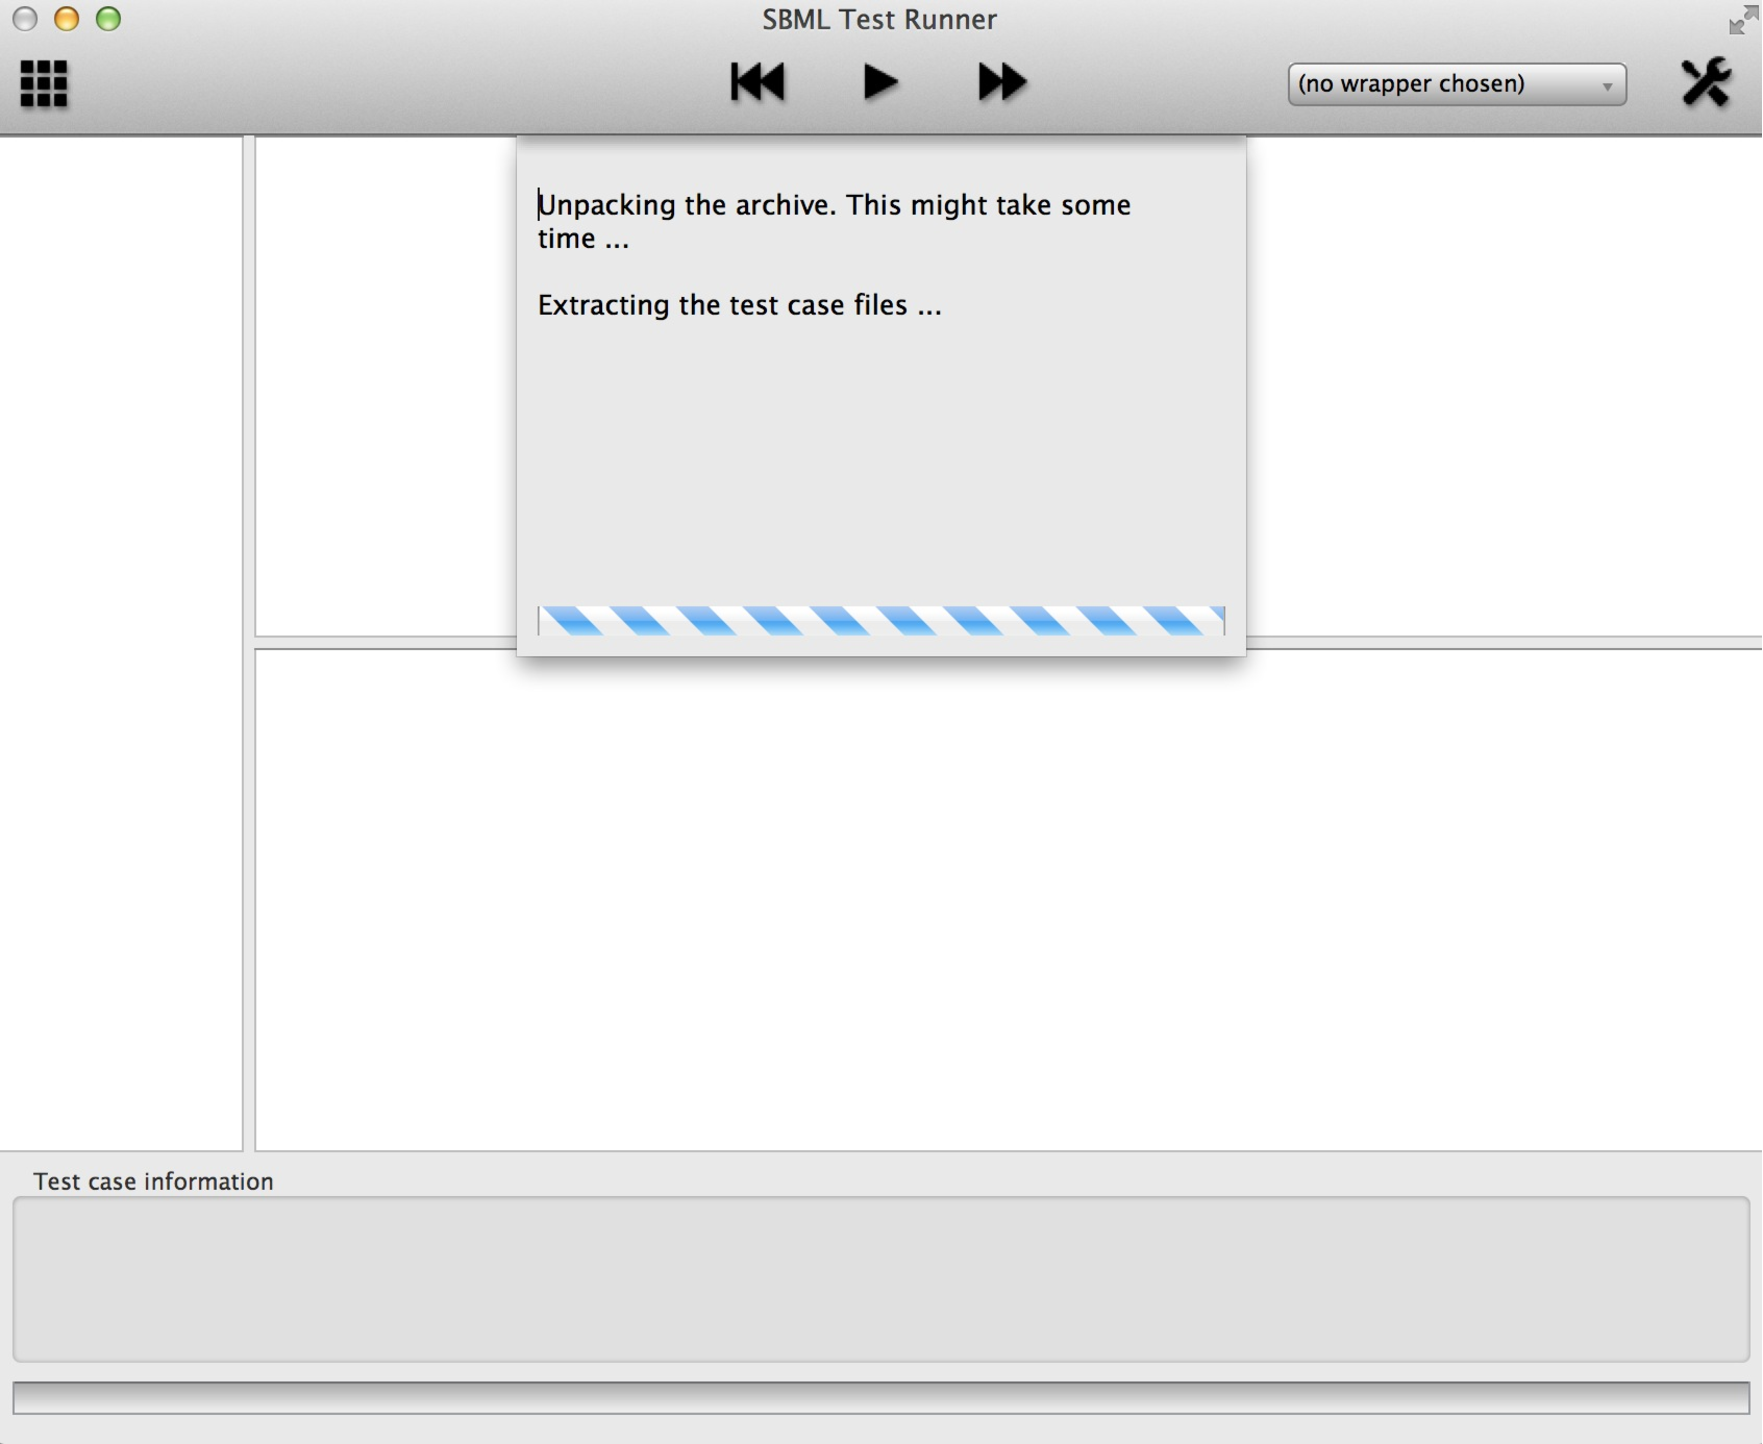
\includegraphics[width = 3.3in]{figs/first-time}}
  \caption{When you first start the SBML Test Runner, it will begin to unpack the SBML test cases it contains internally.  This may take some time, during which it will display a panel describing what it is doing.}
  \label{first-time}
\end{figure}

After this initial unpacking of test cases, the system will not have to do that process again, unless you update the test cases using the Open option in the File menu or change the path to where the SBML Test Runner looks for the cases.  The latter is determined by the Preferences panel, discussed below.


\subsection{Configuring an application wrapper}

The SBML Test Runner will initially not have any wrapper definitions available.  After the Test Runner finishes unpacking the test archive described above, you will be faced with a blank screen and the wrapper selection menu will have the text ``(no wrapper chosen)'' shown on it.  To define a wrapper, click the tool-shaped icon shown in the upper right-hand corner of the application window, or select the Preferences menu item from the application menu.  This will display the Preferences panel, an image of which is shown in \fig{preferences-1}.

\begin{figure}[hbt]
  \fbox{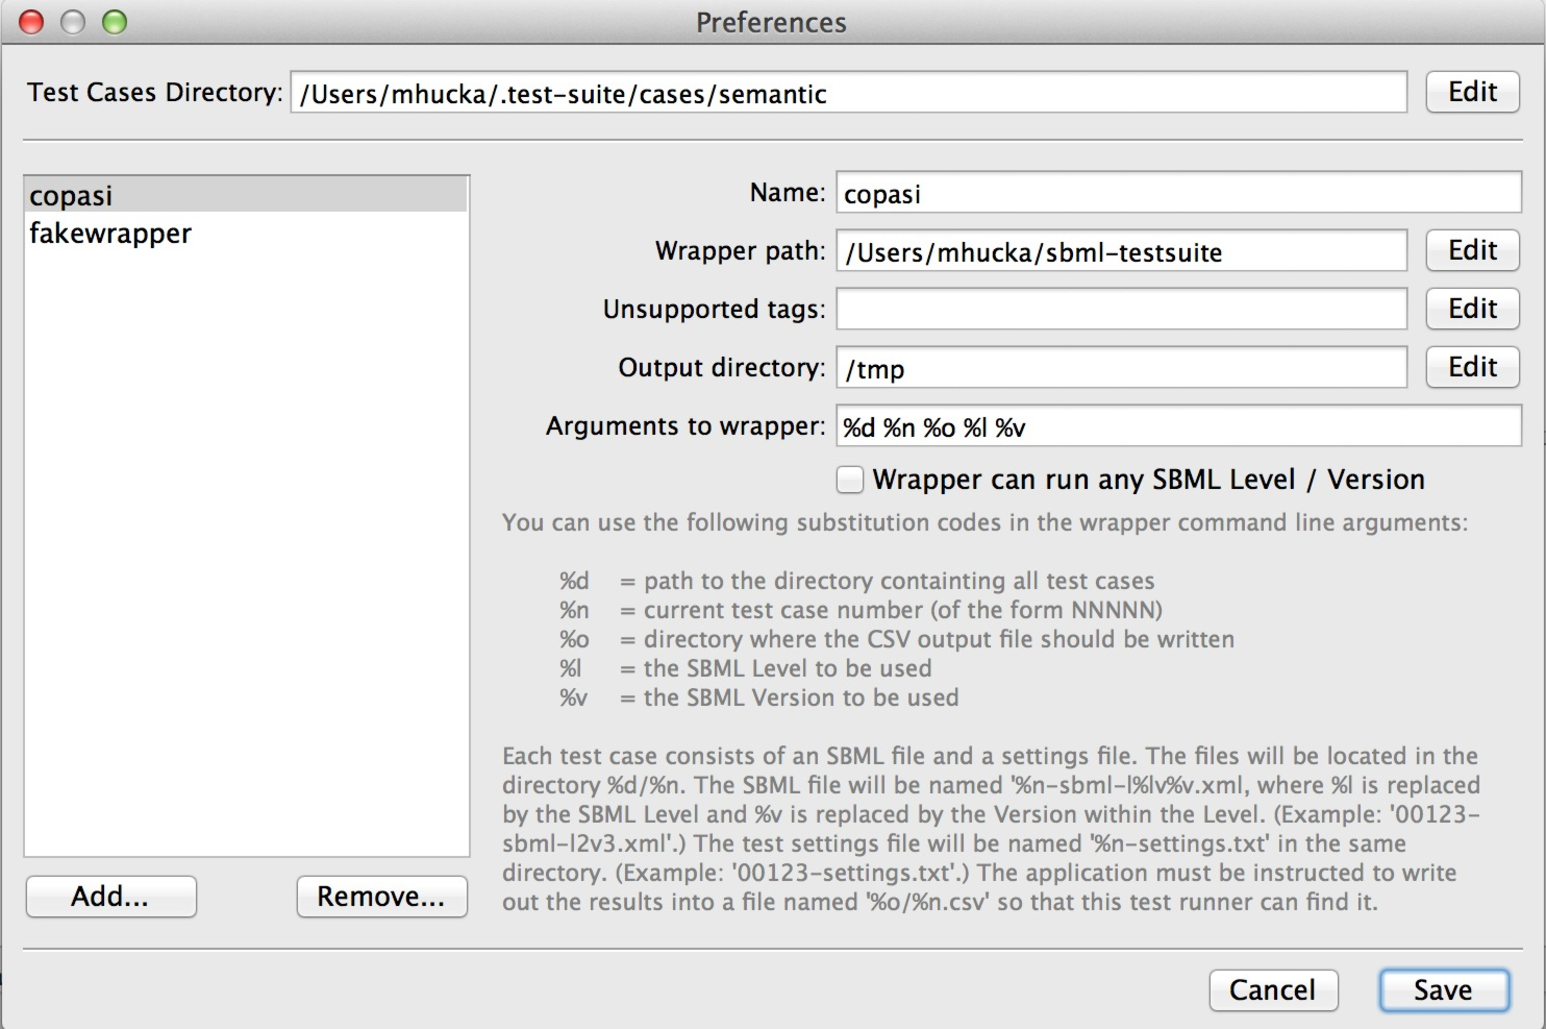
\includegraphics[width = 3.25in]{figs/preferences-1}}
  \caption{The Preferences dialog.}
  \label{preferences-1}
\end{figure}

The first line, titled \emph{Test Cases Directory}, will be automatically pre-configured with a path to a user data folder where the archive of test cases is unpacked.  You should not need to change this value except in special circumstances.

The middle portion of the panel is concerned with the definition of wrappers.  The list in the left-hand side permits you to define more than one wrapper; this can be useful, for example, if you are testing an application using different options, or testing different applications.   The Add and Remove buttons enable you to manage the list of known wrappers.  The list will be shown in a drop-down menu in the toolbar of the main SBML Test Runner window once you exit the Preferences dialog.

The set of fields to the right of the list of wrappers are the ones that let you define the characteristics of an individual wrapper.  Here are the fields and their meanings:

\begin{description}[style=multiline,leftmargin=1.4in]

\item[Name] This is a name you chose for the wrapper.  It will initially have the placeholder text ``newWrapper'', which you can edit to be anything you find meaningful for your purposes.

\item[Wrapper path] The full path to the wrapper program. You can click the ``Edit'' button to the right of the field to invoke a file dialog box that will let you select the program on your file system.

\item[Unsupported tags] These are test tags or component tags that represent test features that are known not to be supported by the application.  You can click the ``Edit'' button next to the field to bring up the tag selection dialog shown in \fig{tag-selection}.

\begin{figure}[h]
  \fbox{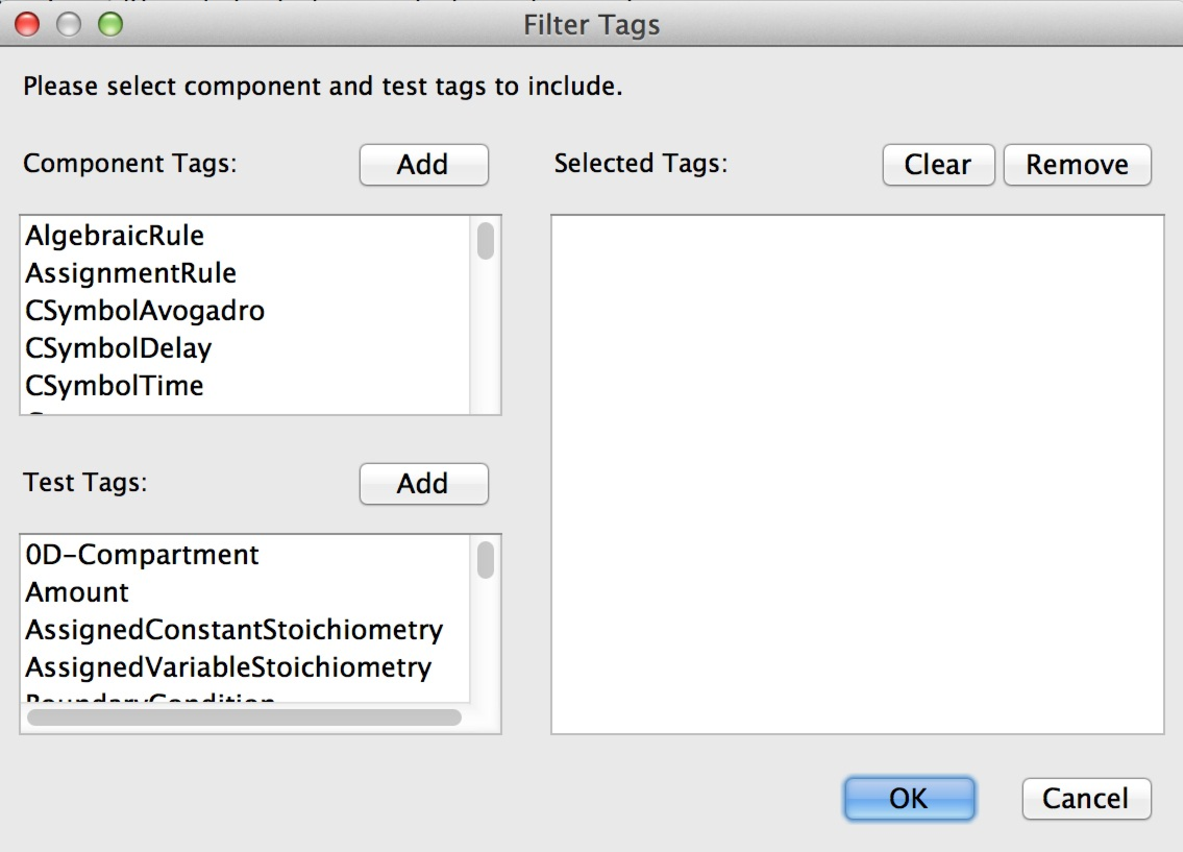
\includegraphics[width = 2.25in]{figs/tag-selection}}
  \caption{The dialog for selecting unsupported test and component tags.}
  \label{tag-selection}
\end{figure}

\item[Output directory] This is a directory where the application will be instructed to write the output files (as comma-separated value \texttt{.csv} files) generated by running each test case.  A typical choice might be \texttt{/tmp} on Linux and Unix-like systems.  As with the other fields, you can click the ``Edit'' button next to the field to bring up a file navigation dialog, which you can then use to select a directory on your file system.

\item[Arguments to wrapper] In order to convey to the wrapper (and the underlying application) such things as the current test case, the command line executed for running the wrapper can include certain substitution codes.  These codes are sequences of characters that will be replaced with actual values at the time the wrapper is invoked for a given test case.  The possible substitution codes are summarized in \tab{substitutions}.

\begin{table}[t]
  \rowcolors{2}{sbmlrowgray}{}
  \begin{tabular}{cl}
    \toprule
    \textbf{Code} & \textbf{Meaning} \\
    \midrule
    \texttt{\%d} & The path to the directory where all the cases are located.
    \\
    \texttt{\%n} & The current test number (a five-digit number).
    \\
    \texttt{\%o} & The path to the directory where the output of should be written by the application.
    \\
    \texttt{\%l} & The level of the SBML file.
    \\
    \texttt{\%v} & The version of the SBML file.
    \\
    \bottomrule
  \end{tabular}
  \caption{The substitution codes that can be used in wrapper command lines.}
  \label{substitutions}
\end{table}


\item[Wrapper can run any SBML Level/Version] This checkbox can be used to indicate that the wrapper supports all Levels and Versions of SBML.

\end{description}

The wrapper is really an adaptor, an interface.  Usually, a wrapper will need to incorporate the ability to parse the \texttt{NNNNN-settings.txt} file found in each SBML Test Suite test case, and to communicate some or all of the values in that file to the application being tested.  The settings file contains information about such things as the duration of the simulation to run, numeric tolerances, the number of time steps to produce output for, the variables whose values should be writing to the output file, and more.  Given the basic information handed to it by the SBML Test Runner (i.e., the values communicated using the substitution codes of \fig{substitutions}), the wrapper needs to find the settings file, read it, determine what needs to be communicated to the application, and invoke the application in a suitable way.

The wrapper may also need to take the output produced by the application being tested and reformat it to produce the output required by the SBML Test Runner.  The output of a test will be numerical values for variables indicated in the \texttt{NNNNN-settings.txt} file, and these values need to be written to a comma-separated value file that will then be read by the SBML Test Runner itself.  Depending on the application, it may be the application itself that writes the results in the necessary format, or the wrapper may need to take whatever output is produced by the application and turn it into the comma-separated value file needed by the Test Runner.

Once you have configured at least one wrapper, click the Save button in the Preferences dialog to return to the main SBML Test Runner application window.


\subsection{The basics of running tests}

\fig{main-window} shows a screen image of the main SBML Test Runner window, with labels to help identify the different parts.  You will no doubt quickly understand the way the different elements work simply through experimentation, but a few features bear explanation.

\begin{figure}[hb]
  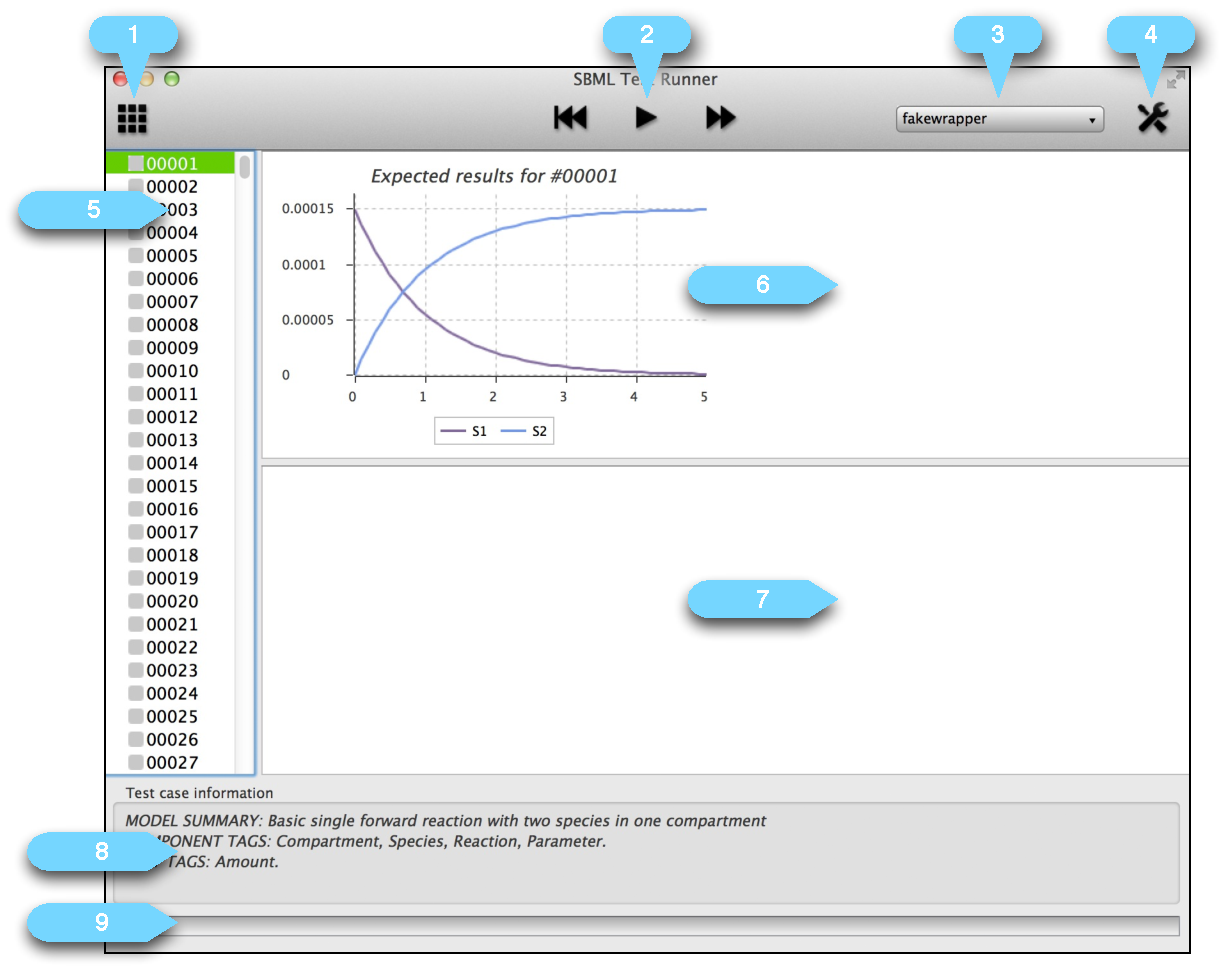
\includegraphics[width = 4.5in]{figs/main-window-illustration}
  \caption{The main window and its different constituents.  (1) The Map View button.  (2) The run control buttons.  (3) The wrapper selection pull-down menu.  (4) The Preferences button.  (5) The list of test cases currently defined.  (6) Two graphs, the one on the left representing the expected results and the one on the right (when there is one) representing the results produced by the application being tested.  (7) A plot of the differences between the two results shown in (6), when there is a result to show.  (8) Status area, used to show a summary of the test case currently selected in the list shown in area (5).  (9) Progress bar for the current run.}
  \label{main-window}
\end{figure}


The toolbar at the top of the window consists of several icons and a pull-down menu; these are the items (1)--(4) shown in \fig{main-window}.  The most basic way to start the tests is to use the run buttons (2).  Their meanings are as follows:

\begin{description}[style=multiline,leftmargin=0.4in]

\item {\hspace*{-0.4in}
\includegraphics[width = 0.25in]{figs/rewind-button}\hspace*{0.1in}} The ``rewind'' button resets the starting point for the next run to case (00001).

\item {\hspace*{-0.4in}
\includegraphics[width = 0.25in]{figs/play-button}\hspace*{0.1in}} The ``run''/''pause'' button starts running tests, and while tests are running, it changes to a pause button.  By default, the ``run'' button runs all tests beginning from the first case (00001); if you select tests by highlighting them in the list shown in area (5) of \fig{main-window}, it will run only that subset of test cases.  While the Test Runner is executing tests, you can click on the ``pause'' button that will appear in place of the ``run'' button to pause execution.  Immediately after you click on ``pause'', the button shape will revert to ``run'' again, thus allowing you to click it to continue running.

\item  {\hspace*{-0.4in}
\includegraphics[width = 0.25in]{figs/fast-play-button}\hspace*{0.1in}} The ``fast run'' button is similar to the regular ``run'' button, except that it causes the Test Runner to skip tests that already have a result.  This can be useful, for example, when changing which tests are excluded via tags.


\end{description}




% \section{Detailed explanations}






\end{document}
